\nocite{MathWorksParallelComputing}
Il \textit{Parallel Computing Toolbox}, spesso abbreviato in PCT, permette di risolvere problemi \textit{data-intensive} e \textit{compute-intesive} sfruttando 
la potenza di calcolo offerta dai microprocessori \textit{multicore} e dai moderni cluster di \textit{elaboratori}. \newline
Costrutti di programmazione di alto livello, come i vettori distribuiti, consentono di sviluppare applicazioni MATLAB scalabili senza ricorrere alla programmazione MPI \footnote{La \textit{Message 
Passing Interface}, o semplicemente MPI, rappresenta lo standard per il modello di comunicazione interprocesso, basato sullo scambio di messaggi, impiegato nelle elaborazioni 
parallele su sistemi distribuiti \cite{NMSUMPIIntro}}.\newline
Inoltre, la stessa applicazione pu\`o essere eseguita su \textit{cluster} o su server in \textit{cloud} senza apportare alcuna modifica al codice grazie a MATLAB 
\textit{Parallel Server}, cos\`i da concentrarsi esclusivamente sullo sviluppo del modello matematico migliore per il caso d'uso in questione.

Incominciamo il nostro studio del PCT riportando alcune definizioni di particolari aspetti del modello di programmazione di MATLAB considerate fondamentali per la prosecuzione della trattazione.
\begin{itemize}
\item \textit{Client}: termine impiegato per identificare la sessione di MATLAB attiva con cui l'utente finale sta interagendo; tipicamente, corrisponde con il \textit{computer} usato dallo sviluppatore durante la prototipazione e lo sviluppo in locale del programma.\newline
Attraverso le funzionalit\`a offerte dal PCT, un \textit{client} pu\`o gestire la computazione da eseguire suddividendola in  task pi\`u semplici e assegnando ciascuna task a un MATLAB \textit{worker}.
\item \textit{Worker}: corrisponde a un'istanza di MATLAB, priva di interfaccia grafica, controllata da un \textit{client} e in grado di fornire la potenza del motore di calcolo del linguaggio.
\item \textit{Parallel Pool}: spesso abbreviato in parpool, \`e un insieme di \textit{worker} comunicanti che possono eseguire codice interattivamente.
\end{itemize}

Una prima distinzione da sottolineare \`e quella tra l'infrastruttura e i componenti del linguaggio esposti dagli strumenti di calcolo parallelo in MATLAB. 
Il linguaggio comprende costrutti di programmazione paralleli e funzioni con supporto automatico al parallelismo mentre l'infrastruttura riguarda i meccanismi 
a supporto del linguaggio, come il protocollo seguito per il trasferimento del codice e dei dati alle unit\`a di lavoro del sistema. \newline
Nelle prossime sezioni, esamineremo da vicino alcuni costrutti paralleli offerti da MATLAB, accennando solamente all'infrastruttura sottostante, nonostante entrambe le componenti siano imprescindibili all'interno del \textit{framework} in questione.

L'architettura di riferimento fino alla fine del capitolo \`e schematizzata in figura \ref{fig:ArchitetturaRiferimento}.\newline
MATLAB \textit{Parallel Server} comprende un insieme di \textit{worker}, in esecuzione sui nodi del \textit{cluster}, che ricevono le 
\textit{task} computazionali dal \textit{client} attraverso specifiche funzioni del \textit{Parallel Computing Toolbox}. \newline
I \textit{worker} prelevano il codice da eseguire e i dati su cui lavorare da una memoria di massa condivisa popolata dall'\textit{head node} (non rappresentato in figura), un nodo speciale eletto all'interno del \textit{cluster} che si occupa dell'assegnazione delle attivit\`a ai \textit{worker} e dell'interfacciamento con il \textit{client}.\newline
Una volta terminata l'elaborazione, i risultati vengono raccolti dal nodo \textit{master} e trasferiti all'interno dello spazio di lavoro del \textit{client} mediante il canale di comunicazione instaurato tra il \textit{client} e MATLAB \textit{Parallel Server}.

\begin{figure}[htbp]
    \centering
    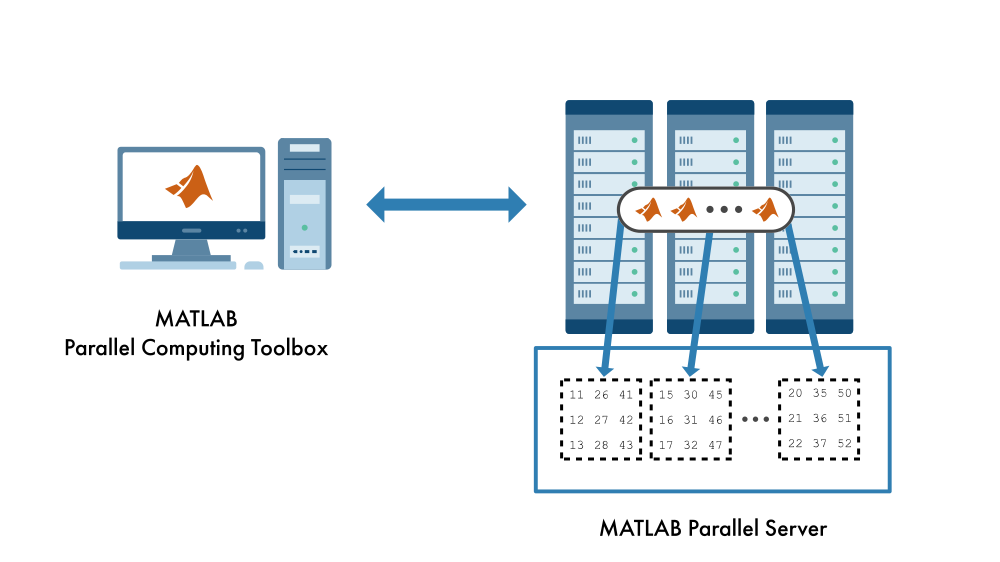
\includegraphics[width=0.8\textwidth]{../Immagini/Capitolo 2/ReferenceArchitecture.png}
    \caption{Architettura di riferimento per gli strumenti di calcolo parallelo in MATLAB. \small{(Da \url{https://it.mathworks.com/products/matlab-parallel-server.html})}}
    \label{fig:ArchitetturaRiferimento}
\end{figure}

A questo punto, accenniamo alle modalit\`a di esecuzione del software parallelo su un sistema multiprocessore supportate dall'ambiente MATLAB:
\begin{itemize}
    \item parallelizzazione implicita: alcune funzioni, se richiamate nel codice sorgente del programma, sfruttano le librerie di \textit{runtime} del linguaggio in modo da essere 
    eseguite su \textit{thread} distinti all'interno della stessa sessione, beneficiando di notevoli miglioramenti di \textit{performance} su sistemi con un numero elevato 
    di processori;
    \item parallelizzazione esplicita: il carico di lavoro del programma viene automaticamente suddiviso in \textit{task} elementari, ciascuna delle quali viene poi assegnata a un \textit{worker} per l'esecuzione.
\end{itemize}

\subsection{Il paradigma di programmazione parallela implicita}
I \textit{toolbox} di MATLAB sono dotati di un crescente numero di funzioni con supporto automatico al parallelismo, al fine di beneficiare di tutti 
i vantaggi propri dall'elaborazione parallela senza modificare i file di codice preesistenti, in accordo con i principi di design elencati nel paragrafo \ref{par2.1}. 

Alcune funzioni, come \lstinline|mldivide| impiegata per la risoluzione di sistemi di equazioni lineari, vengono eseguite in parallelo di \textit{default} se invocate dalla sessione principale di MATLAB. 

Ragionando sulla nostra architettura di riferimento, il \textit{multithreading} implicito viene attivato solo quando la funzione viene eseguita direttamente dal \textit{client}, mentre viene evitato se l'esecuzione \'e a carico dei nodi del \textit{cluster} per evitare un parallelismo \enquote{annidato}, che degraderebbe le prestazioni dell'intero sistema. \newline
In quest'ottica, possiamo notare come i progettisti del linguaggio abbiano pensato a un \textit{worker} come un'unit\`a di elaborazione a singolo \textit{thread}.

Il \textit{client}, quando incontra una funzione con supporto automatico al parallelismo nel codice sorgente del programma, avvia un \textit{parpool} per la sua esecuzione in parallelo. \newline
Un apposito profilo di configurazione determina le caratteristiche dell'ambiente di elaborazione parallela e, in particolare, PCT permette di scegliere tra i seguenti profili preimpostati:
\begin{itemize}
    \item \textit{Processes}: i \textit{worker} vengono attivati come processi indipendenti eseguiti dai \textit{core} fisici del calcolatore su cui \`e attiva la sessione principale di MATLAB.
    \item \textit{Threads}: i \textit{worker} sono ospitati da \textit{thread} e non pi\`u da processi veri e propri. I vantaggi portati da questo ambiente parallelo sono un minor uso di memoria, un basso costo di comunicazione tra i \textit{worker} e uno \textit{scheduling} delle attivit\`a particolarmente performante, a scapito della disponibilit\`a di una ristretta gamma di funzioni con supporto al parallelismo su \textit{thread}.
\end{itemize}
Per quanto riguarda la scelta del numero di \textit{worker} per l'ambiente \textit{Processes}, \'e consigliato riservare un motore di calcolo per ogni \textit{core} fisico disponibile, ignorando la presenza di eventuali \textit{core} virtuali; infatti, questi ultimi condividono alcune risorse di calcolo all'interno dello stesso processore, tra cui la \textit{Floating Point Unit} (FPU), e poich\'e la maggior parte delle elaborazioni in MATLAB richiede l'esecuzione di operazioni aritmetiche in virgola mobile, limitare a uno il numero di \textit{worker} per unit\`a di esecuzione pu\`o aumentare la stabilit\`a del sistema. \newline 
L'unica eccezione \`e rappresentata dalle applicazioni \textit{data-intensive}, per le quali potrebbe essere conveniente portare il numero di \textit{worker} per \textit{core} fisico a due.

In ogni caso, il massimo numero di \textit{worker} presenti in un singolo \textit{parpool} a supporto della parallelizzazione implicita \'e pari a 512, a prescindere dalle specifiche del calcolatore utilizzato.
\begin{figure}[htbp]
    \centering
    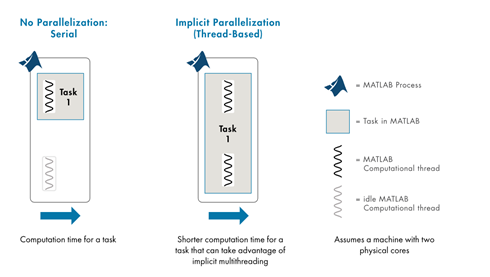
\includegraphics[width=0.8\textwidth]{../Immagini/Capitolo 2/ImplicitParallelization.png}
    \caption{Rappresentazione del modello di parallelizzazione implicita di MATLAB su un sistema \textit{dual-core} \small{(Da \url{https://it.mathworks.com/discovery/matlab-multicore.html})}}
    \label{fig:ParallelismoImplicito}
\end{figure}\newline
Se una funzione non include il supporto automatico al parallelimo, possiamo trasferire l'esecuzione del programma a una \textit{workstation}, in modo da beneficiare dello \textit{speedup} offerto da un sistema con maggiore capacit\`a di calcolo, oppure possiamo utilizzare il paradigma di programmazione parallela esplicita supportato dal \textit{Parallel Computing Toolbox}.

\subsection{Il paradigma di programmazione parallela esplicita}

Il modello di programmazione parallela esplicita in MATLAB conta sulla presenza di costrutti di programmazione parallela a diversi livelli di astrazione.